\documentclass[listings]{labreport}
\usepackage{amsmath}
\usepackage{enumitem}

\usepackage{array}
\newcolumntype{L}[1]{>{\raggedright\let\newline\\\arraybackslash\hspace{0pt}}m{#1}}

\subject{Тестирование программного обеспечения}
\titleparts{Лабораторная работа №4}{Нагрузочное и стресс-тестирование}
\students{Лабушев Тимофей}

\begin{document}

\maketitlepage

\section*{Задание}

С помощью программного пакета \textit{Apache JMeter} провести нагрузочное и
стресс-тестирование веб-приложения в соответствии с вариантом задания.

В ходе нагрузочного тестирования необходимо протестировать 3 конфигурации
аппаратного обеспечения и выбрать среди них наиболее дешёвую, удовлетворяющую
требованиям по максимальному времени отклика приложения при следующей нагрузке:
\begin{enumerate}[noitemsep,topsep=0em]
\item максимальное количество параллельных сессий — 14;
\item средняя нагрузка, формируемая одной сессией — 20 запросов в минуту;
\item максимально допустимое время обработки запроса — 880 мс.
\end{enumerate}
\vspace{0.4em}

При выборе конфигурации принять следующие стоимости:
\begin{itemize}[noitemsep,topsep=0em]
\item Конфигурация 1 — \$2100
\item Конфигурация 2 — \$3200
\item Конфигурация 3 — \$3800
\end{itemize}

В ходе стресс-тестирования необходимо определить, при какой нагрузке
выбранная на предыдущем шаге конфигурация перестаёт удовлетворять требованиям
по максимальному времени отклика. Для этого необходимо построить график зависимости
времени отклика приложения от нагрузки.

\section*{Тестовой план JMeter для нагрузочного тестирования}

Структура тестового плана:
\begin{itemize}[noitemsep,topsep=0em,label=$\bullet$]
  \item Thread Group (Number of Threads: 14, Loop Count: 50)
    \begin{itemize}[noitemsep,topsep=0em,label=$\bullet$]
      \item HTTP Request (\verb|http://...&conf=1|)
        \begin{itemize}[noitemsep,topsep=0em,label=$\bullet$]
          \item Constant Throughput Timer (20 samples per minute)
        \end{itemize}
    \end{itemize}
\end{itemize}
\begin{itemize}[noitemsep,topsep=0em,label=$\bullet$]
  \item Thread Group (Number of Threads: 14, Loop Count: 50)
    \begin{itemize}[noitemsep,topsep=0em,label=$\bullet$]
      \item HTTP Request (\verb|http://...&conf=2|)
        \begin{itemize}[noitemsep,topsep=0em,label=$\bullet$]
          \item Constant Throughput Timer (20 samples per minute)
        \end{itemize}
    \end{itemize}
\end{itemize}
\begin{itemize}[noitemsep,topsep=0em,label=$\bullet$]
  \item Thread Group (Number of Threads: 14, Loop Count: 50)
    \begin{itemize}[noitemsep,topsep=0em,label=$\bullet$]
      \item HTTP Request (\verb|http://...&conf=2|)
        \begin{itemize}[noitemsep,topsep=0em,label=$\bullet$]
          \item Constant Throughput Timer (20 samples per minute)
        \end{itemize}
    \end{itemize}
\end{itemize}

Для запуска тестового плана использовалась следующая команда:

\verb|apache-jmeter-5.3/bin/jmeter -n -t load-test.jmx -l load-test.csv|

Где \verb|load-test.jmx| — файл конфигурации тестового плана,
\verb|load-test.csv| — файл с выходными значениями, в который
записываются показатели каждого отправленного запроса.

\newpage
\section*{Результаты нагрузочного тестирования}

По собранным данным составим сравнительную таблицу конфигураций:

\renewcommand{\arraystretch}{1.5}
\noindent
\begin{tabular}{|L{3cm}|L{5cm}|L{5cm}|L{3cm}|} 
\hline
Конфигурация & Максимальное время обработки запроса, мс & Среднее время обработки запроса, мс & Стоимость \\\hline
1 & 2296 & 757 & \$2100 \\\hline
2 & 767 & 553 & \$3200 \\\hline
3 & 524 & 354 & \$3800 \\\hline
\end{tabular}

Максимальное время обработки запроса при использовании первой конфигурации
в разы превышает требования к системе, однако среднее время обработки запроса
им удовлетворяет.

Чтобы убедиться, что высокий показатель не был единичным случаем, построим
график изменения времени обработки запросов на протяжении теста:

\vspace{0.4em}
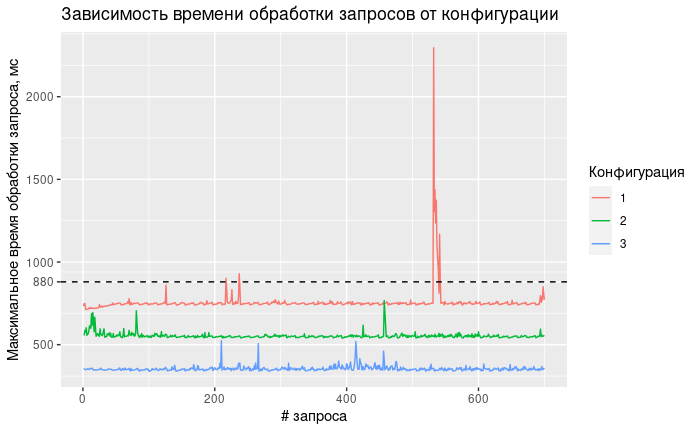
\includegraphics[width=0.8\textwidth]{Lab4/Load-Test-Plot.png}

Можем увидеть, что при использовании первой конфигурации превышение максимально
допустимого времени происходит многократно. Таким образом,
\textbf{оптимальной является вторая конфигурация}, которая удовлетворяет
требованиям и имеет меньшую стоимость по сравнению с третьей.

\newpage
\section*{Тестовой план JMeter для стресс-тестирования}

Стресс-тестирование произведено для второй конфигурации, которая была выбрана
как наиболее дешевая, при этом удовлетворяющая заданным требованиям.

Структура тестового плана:
\begin{itemize}[noitemsep,topsep=0em,label=$\bullet$]
  \item Thread Group (Number of Threads: 200, Ramp-up period: 90 seconds)
    \begin{itemize}[noitemsep,topsep=0em,label=$\bullet$]
      \item HTTP Request (\verb|http://...&conf=2|)
        \begin{itemize}[noitemsep,topsep=0em,label=$\bullet$]
          \item Constant Throughput Timer (20 samples per minute)
        \end{itemize}
    \end{itemize}
\end{itemize}

Тестовый план запускается следующей командой:

\verb|apache-jmeter-5.3/bin/jmeter -n -t load-test.jmx -l load-test.csv|

\section*{Результаты стресс-тестирования}

Построим график зависимости максимального и среднего времени обработки запросов
от числа одновременных пользователей:

\vspace{0.4em}
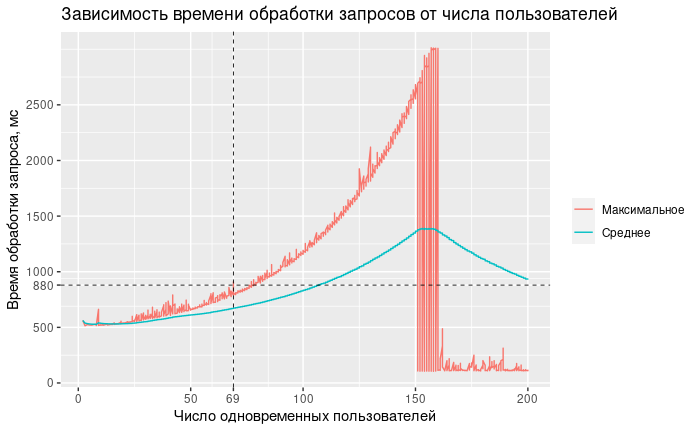
\includegraphics[width=0.8\textwidth]{Lab4/Stress-Test-Response-Time-Plot.png}

Начиная с \textbf{69} одновременных пользователей, система прекращает удовлетворять
требованиям к максимальному времени обработки запроса. Среднее время обработки
запроса продолжает оставаться ниже 880 мс в пределах 100 пользователей.

При достижении 150 пользователей наблюдается странный эффект: время обработки
запросов резко падает. Объяснение подобному поведению можно найти, построив
график частоты ошибок, возвращаемых сервером:

\vspace{0.4em}
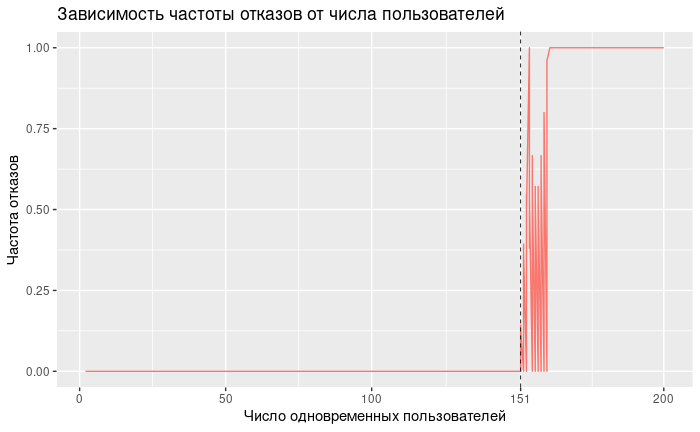
\includegraphics[width=0.8\textwidth]{Lab4/Stress-Test-Error-Rate-Plot.png}

Начиная со 151 одновременного пользователя выбранная конфигурация не справляется
с нагрузкой и начинает отказывать в обслуживании, возвращая ошибки \verb|HTTP 503|.

\section*{Исходный код}

\verb|https://github.com/timlathy/itmo-fourth-year/tree/master/Software-Testing-7th-Term/Lab4|

\section*{Выводы}

В ходе выполнения работы был рассмотрен инструмент для проведения нагрузочного тестирования
\textit{Apache JMeter}. Было произведено сравнение трех конфигураций на основании данных,
собранных в ходе тестирования, и принято решение о выборе оптимальной из них.

Для выбранной конфигурации также было произедено стресс-тестирование, в ходе чего было
определено максимальное количество одновременных пользователей, удовлетворяющих требованиям,
а также число пользователей, при котором система начинает отказывать в обслуживании.

\end{document}
